\documentclass[12pt]{article}
\usepackage[spanish]{babel }
\usepackage{graphicx}
\usepackage{float}
\usepackage{hyperref}
\usepackage{times}
%opening
\title{\textbf{\textit{\underline{¿Inundación o sequía?}}}}

\begin{document}
	
\begin{titlepage}
	\centering
	\vspace*{1cm}
	\begin{figure}
		\centering
		
\includegraphics[width=0.3\linewidth]{images/logo}
		\label{fig:logo}
	\end{figure}
	
	\large{\textbf{Universidad de La Habana}\\
	Facultad de Matemática y Computación\\}
	\vspace{3.5cm}
	
	{\rmfamily\selectfont\Huge{¿Inundaciones o sequía?}} 
	\vspace{1.5cm}
	
	\Large
	\vspace{2 cm}
	\normalsize{\textbf{Autores:}\\
		Jennifer de la Caridad Sánchez Santana\\
		Angélica María Martínez Céspedez\\
		Guillermo Ferriol Ravelo\\
		Diego Puentes Fernández\\}
	\vfill
	
	\large
	\today
\end{titlepage}

	
	\begin{center}
		\textbf{\textit{\underline{{\fontsize{60}{24}\selectfont Huracán Ian:}}}}
	\end{center}
	
	
	\begin{figure}[H]
		\centering
		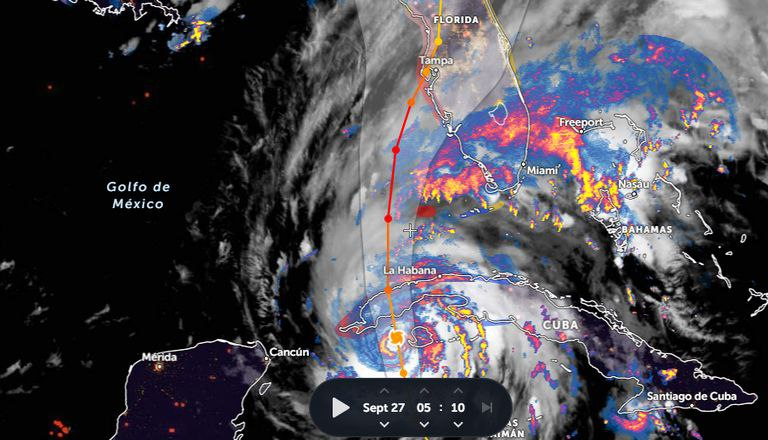
\includegraphics[width=0.7\linewidth]{./Report/images/Ian}
		\label{fig:ian}
	\end{figure}
	
	
	A las 4:40 de la madrugada del día 27 de septiembre del 2022, tocaba tierras cubanas por la provincia de Pinar del Río, un intenso huracán de nombre Ian, con vientos máximos sostenidos de 205 km/h, y de categoría "3" según la escala Saffir-Simpson. Durante la mañana de este mismo día, ocurrieron en dicha provincia vientos fuertes en racha y numerosas lluvias, así como inundaciones costeras hacia la costa sur. A las 9:50 am, Ian emergió al sudeste del Golfo de México, quedando aún en algunos pueblos, vientos sostenidos de 185 km/h. Ya en la tarde, había dejado totalmente la Isla, adentrándose cada vez más en aguas del golfo. En tan solo 7 horas, el huracán provocó graves daños en las redes principales y secundarias de suministro de agua, y en sistemas de abastecimiento de varios municipios, también ocasionó derrumbes parciales y totales en miles de viviendas, afectaciones a las coberturas e infraestructura de instituciones públicas y conjuntamente al suministro de electricidad en el país, además, generó caída de árboles, inundaciones en zonas bajas y cuantiosos daños en la agricultura.\cite{webpage1}
	
	
	\begin{figure}[H]
		\centering
		\includegraphics[width=0.6\linewidth]{./Report/images/huracán_Ian}
		\caption{Huracán Ian.}
		\label{fig:huracanian}
	\end{figure}
	
	Una vez que el huracán Ian dejó de ser una amenaza, se pudo constatar la magnitud de los daños y determinar las provincias que sufrieron mayor impacto, siendo Pinar del Río, Artemisa, Mayabeque y La Habana las más afectadas. Con la excepción de Mayabeque, todas estas localidades experimentaron precipitaciones por encima de la media, no obstante, esto no cambia el hecho de que el resto del país estuviera en medio de una extensa desecación, y por si fuera poco, a pesar de que en el mes de octubre las copiosas inundaciones y precipitaciones ocasionadas por el huracán fueron prominentes, las áreas mencionadas con anterioridad experimentaron una severa sequía, evidenciando la dualidad de la naturaleza y su impacto en nuestras vidas.\cite{webpage2}
	
	
	
	\begin{figure}[H]
		\centering
		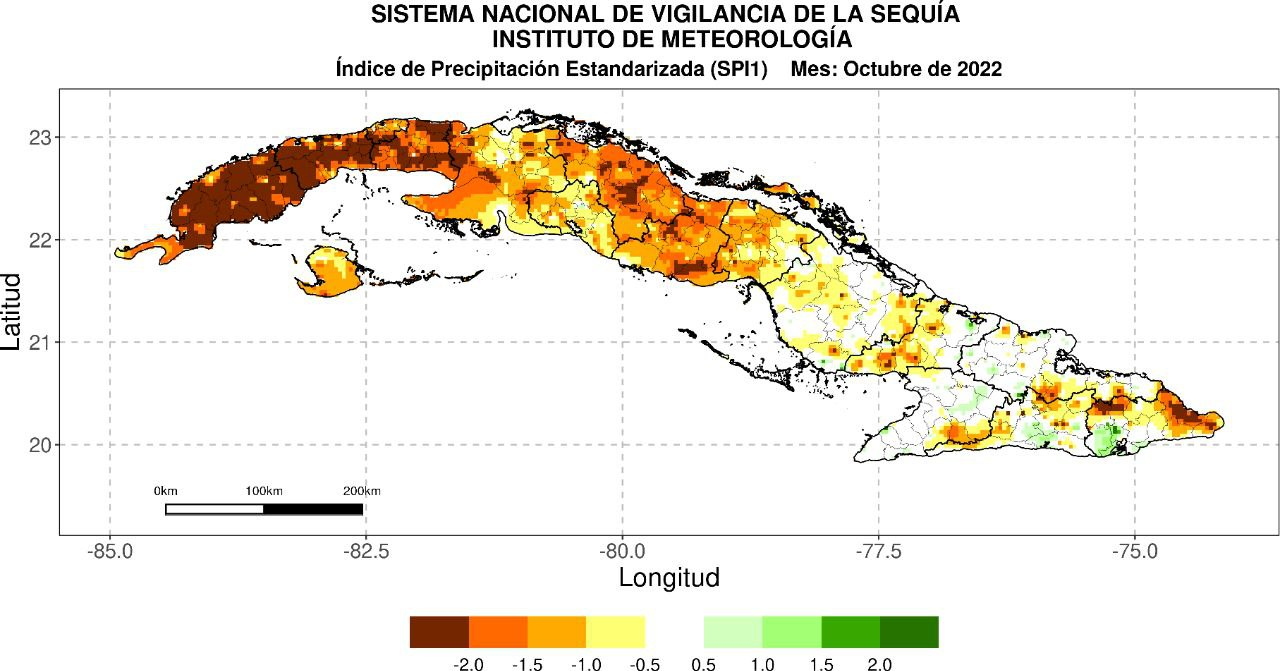
\includegraphics[width=0.8\linewidth]{./Report/images/mapa_octubre_ismet}
		\caption{Mapa de Cuba con las provincias más afectadas en el mes de octubre.}
		\label{fig:mapaoctubreismet}
	\end{figure}
	
	\begin{figure}[H]
		\centering
		\includegraphics[width=0.7\linewidth]{./Report/images/provincias_más_afectadas}
		\caption{Comportamiento de las precipitaciones en las provincias más afectadas.}
		\label{fig:provinciasmasafectadas}
	\end{figure}
	
	
	
	\begin{figure}[H]
		\centering
		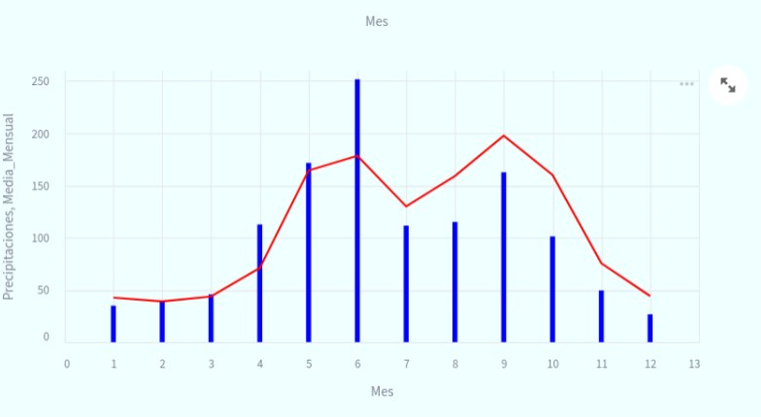
\includegraphics[width=0.8\linewidth]{./Report/images/precipitaciones_2022}
		\caption{Comportamiento de las precipitaciones por mes en 2022.}
		\label{fig:precipitaciones2022}
	\end{figure}
	
	
	\newpage
	En este contexto, resulta paradójico que los territorios que sufrieron los estragos e inundaciones causados por el tránsito de Ian, coinciden exactamente con aquellos que atravesaron una aguda sequía. Este evento plantea la cuestión de si los fenómenos naturales que han acontecido en Cuba, generando desde intensas precipitaciones hasta desbordamientos, suministran la cantidad necesaria de agua para contrarrestar esta sequía.\\
	
	Se ha documentado que las sequías más severas de este siglo tuvieron lugar durante períodos específicos, es decir, de 2003-2005, de 2009-2010 y de 2014-2015. Asimismo, durante estos períodos, diversas provincias sufrieron el impacto de intensos ciclones, que desencadenaron inundaciones de gran escala y desastres de notable magnitud.\cite{webpage3}
 
	
	\begin{itemize}
		\item\textbf{Período 2003-2005:}
	\end{itemize}
	
	\begin{figure}[H]
		\centering
		\includegraphics[width=0.9\linewidth]{./Report/images/gráfica_ismet}
		\caption{Tabla del ISMET}
		\label{fig:graficaismet}
	\end{figure}
	
	En el período de 2003 a 2005 se registraron tres tormentas tropicales, una de categoría "3", y las otras dos de categoría "4", conforme a la escala Saffir-Simpson. Estos eventos climáticos provocaron inundaciones en varias provincias, entre las que se incluyen Santiago de Cuba, Matanzas y la Isla de la Juventud.\cite{webpage4}
	
	
	\begin{figure}[H]
		\centering
		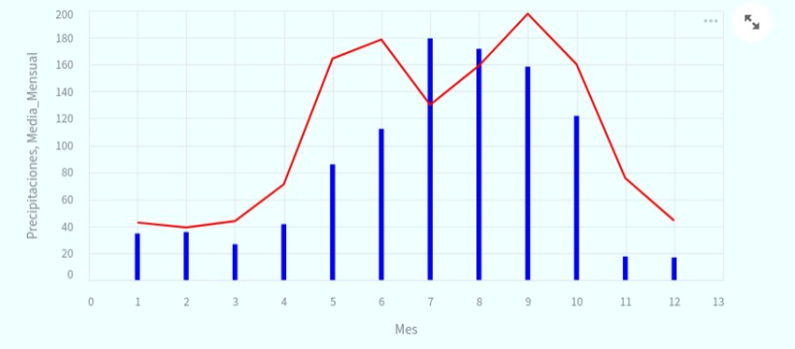
\includegraphics[width=0.7\linewidth]{./Report/images/precipitaciones_2004}
		\caption{Comportamiento de las precipitaciones en 2004.}
		\label{fig:precipitaciones2004}
	\end{figure}
	
	
	\begin{figure}[H]
		\centering
		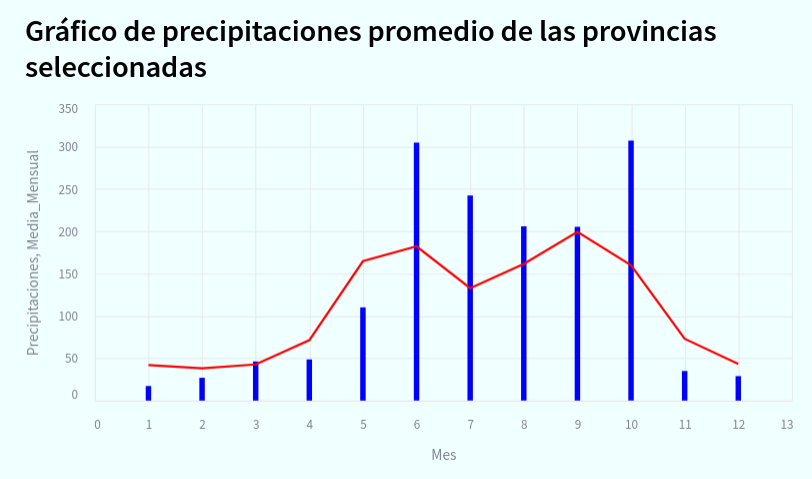
\includegraphics[width=0.7\linewidth]{./Report/images/precipitaciones_2005}
		\caption{Comportamiento de las precipitaciones en 2005.}
		\label{fig:precipitaciones2005}
	\end{figure}
	
	Durante ese mismo lapso de tiempo, se presenció  una de las sequías más intensas  documentadas en los los últimos 50 años.\cite{webpage5}
	
	
	\begin{figure}[H]
		\centering
		\includegraphics[width=0.8\linewidth]{./Report/images/tabla_peligro_sequía}
		\caption{Tabla de peligro de sequía.}
		\label{fig:tablapeligrosequia}
	\end{figure}
	
	\begin{itemize}
		\item\textbf{Período 2009-2010:}
	\end{itemize}
	
	En el año 2009, Cuba experimentó una temporada ciclónica muy inactiva, con escasa presencia de fenómenos naturales. En contraste, en el 2010, la "Depresión Tropical Paula", azotó al país, generando abundantes precipitaciones en la región central. Estas lluvias resultaron favorables para dicha región, ya que contribuyeron a aliviar los efectos de la sequía, al menos durante ese mes y en esa área específica.\cite{webpage6}\cite{webpage7}
	
	\begin{figure}[H]
		\centering
		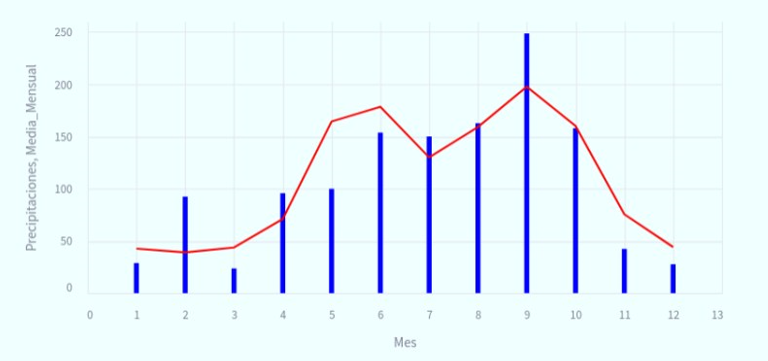
\includegraphics[width=0.6\linewidth]{./Report/images/precipitaciones_2010}
		\caption{Comportamiento de las precipitaciones en el 2010.}
		\label{fig:precipitaciones2010}
	\end{figure}
	
	
	\begin{figure}[H]
		\centering
		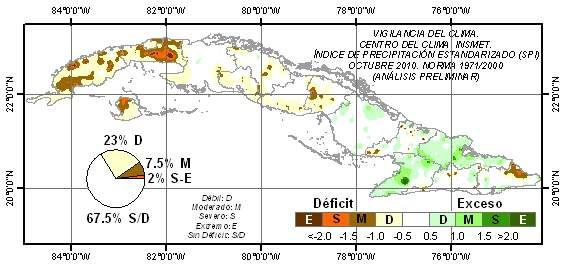
\includegraphics[width=0.7\linewidth]{./Report/images/mapa}
		\caption{Mapa de Cuba de precipitación de octubre del 2010}
		\label{fig:mapa}
	\end{figure}
	
	\begin{itemize}
		\item \textbf{Período 2014-2015:}
	\end{itemize}
	
	El año 2014 mostró un comportamiento similar al año 2009. Sin embargo, en 2015, el huracán "Joaquín", a pesar de no atravesar directamente la Isla, afectó a varias provincias, desde Ciego de Ávila hasta Guantánamo. Este fenómeno metereológico desencadenó intensas lluvias, tormentas eléctricas, marejadas e inundaciones costeras en los primeros días de octubre. Estas precipitaciones jugaron un papel esencial en la  mitigación de los efectos de la sequía en dichos territorios.\cite{webpage6}\cite{webpage8}
	
	\begin{figure}[H]
		\centering
		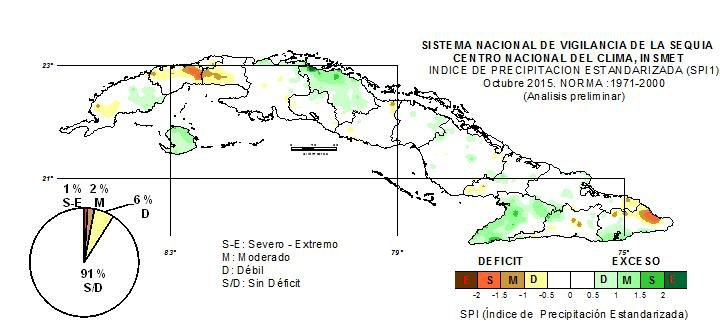
\includegraphics[width=0.7\linewidth]{./Report/images/mapa_octubre_2015}
		\caption{Mapa de Cuba de precipitación de octubre del 2015.}
		\label{fig:mapaoctubre2015}
	\end{figure}
	
	En resumen, la interacción entre los huracanes, las inundaciones y los períodos de sequía en Cuba representa desafíos considerables para la gestión del agua y la adaptación al cambio climático. A pesar de las fuertes lluvias asociadas a los huracanes, las provincias afectadas por estos eventos continúan sufriendo sequías, lo que destaca la complejidad de los impactos climáticos en la disponibilidad de agua. Además, la necesidad de estrategias sostenibles para la gestión de los recursos hídricos y la adaptación a la variabilidad climática se hace cada vez más urgente. Al analizar sucesos pasados y comprender sus repercusiones, se pueden obtener lecciones valiosas para enfrentar los futuros desafíos climáticos y garantizar la seguridad hídrica en Cuba. Es primordial recordar la importancia de cuidar nuestro planeta, nuestra tierra, y contribuir a su preservación de todas las formas posibles. ¡Conserva el agua!
	
	
	\begin{figure}[H]
		\centering
		
\includegraphics[width=0.4\linewidth]{./Report/images/agua}
		\label{fig:agua}
	\end{figure}
	
	
	\newpage
	\begin{thebibliography}{8}
		\bibitem{webpage1} 
		\url{chttps://www.unicef.org/cuba/huracan-ian-cuba}
		
		\bibitem{webpage2}
		\url{http://www.insmet.cu/asp/genesis.asp?TB0=PLANTILLAS&TB1=sqCLIMA&TB2=/clima/Sequia/SQOCTUBRE2015.HTM&TB3=2015}
		
		\bibitem{webpage3}
		\url{https://periodismodebarrio.org/2023/11/las-sequias-en-cuba-explicadas/amp/}
		
		\bibitem{webpage4}
		\url{https://rcm.insmet.cu/index.php/rcm/article/view/493/768}
		
		\bibitem{webpage5}
		\url{http://rcm.insmet.cu/index.php/rcm/article/download/186/127/0
			http://rcm.insmet.cu/index.php/rcm/article/download/186/127/0}
		
		\bibitem{webpage6}
		\url{http://www.insmet.cu/asp/genesis.asp?TB0=PLANTILLAS&TB1=TEMPORADA&TB2=/Temporadas/temporada2020.html}
		
		\bibitem{webpage7}
		\url{http://www.cubadebate.cu/temas/medio-ambiente-temas/2010/11/30/termina-hoy-la-activa-temporada-ciclonica-del-2010/amp/}
		
		\bibitem{webpage8}
		\url{http://www.cubadebate.cu/noticias/2015/10/01/nota-informativa-no-1-del-estado-mayor-nacional-de-la-defensa-civil-sobre-el-huracan-joaquin/amp/}
		
	\end{thebibliography}
	
	
\end{document}